\documentclass[11pt,a4paper]{article}

% --------------------- Packages ---------------------
\usepackage[a4paper,margin=1in]{geometry}
\usepackage[T1]{fontenc}
\usepackage[utf8]{inputenc}
\usepackage{lmodern}
\usepackage{setspace}
\usepackage{microtype}
\usepackage{amsmath,amssymb,amsthm,mathtools}
\usepackage{bm}
\usepackage{physics}
\usepackage{graphicx}
\usepackage{subcaption}
\usepackage{bbm}
%\renewcommand\thesubfigure{\thefigure\alph{subfigure}}
\usepackage{float}
\usepackage{caption}
\usepackage{booktabs}
\usepackage{enumitem}
\usepackage[hidelinks]{hyperref}
\usepackage[nameinlink,capitalize]{cleveref}
\usepackage{cancel}
\usepackage{comment}
\usepackage{algorithm}
\usepackage{algpseudocode}
\usepackage{needspace}

\usepackage{cellspace}
\setlength\cellspacetoplimit{6pt}    % Espace vide au-dessus
\setlength\cellspacebottomlimit{6pt} % Espace vide en-dessous

% --------------------- Formatting ---------------------
\numberwithin{equation}{section}
\setlist[itemize]{topsep=2pt,itemsep=2pt,parsep=0pt}
\setlist[enumerate]{topsep=2pt,itemsep=2pt,parsep=0pt}
\onehalfspacing

\begin{document}

% ----- Title Page -----
\newgeometry{top=2.5cm,bottom=2.5cm,left=2.5cm,right=2.5cm}
\begin{titlepage}
    \centering
    
\includegraphics[width=6cm]{images/EPFL_Logo.png} \\
    \vspace{0.3cm}
    {\LARGE \bfseries ÉCOLE POLYTECHNIQUE\\
    FÉDÉRALE DE LAUSANNE\par}
    \vspace{1cm}
    
    \noindent\rule{\textwidth}{0.4pt}
    {\LARGE \bfseries Meta-Learning NN-control\\on Crazyflie Quadcopter\par}
    
    \noindent\rule{\textwidth}{0.4pt}
    \vspace{1cm}
    
    {\Large \bfseries SEMESTER PROJECT\par}
    \vspace{0.5cm}
    
    {\large \bfseries DECODE \par}
    \vspace{2 cm}
    
    \noindent
    \begin{minipage}[t]{0.5\textwidth}
        {\large \textit{Student:}\\
        Niels Rigaud\\
        SCIPER: 341284\par}
    \end{minipage}%
    \hfill
    \begin{minipage}[t]{0.45\textwidth}
        \raggedleft
        {\large \textit{Professor:}\\
        G. Ferrari Trecate \par}
    \end{minipage}
    \vspace{1.5cm}
    
    {\large \textit{Supervisors:}\\
    Simone Baratto\\Nicolas Kirsch\\Daniele Martinelli}
    \vfill
    
    {\large Spring 2026\par}
\end{titlepage}
\restoregeometry

\pagenumbering{roman}

\tableofcontents
\cleardoublepage
\pagenumbering{arabic}

% =====================================================
\section{Introduction}
\subsection{Motivation}
\subsection{Prior Work}
\subsection{Contributions}

% =====================================================
\section{Background}
\subsection{Quadcopter Dynamics}

\begin{figure}[H]
    \centering
    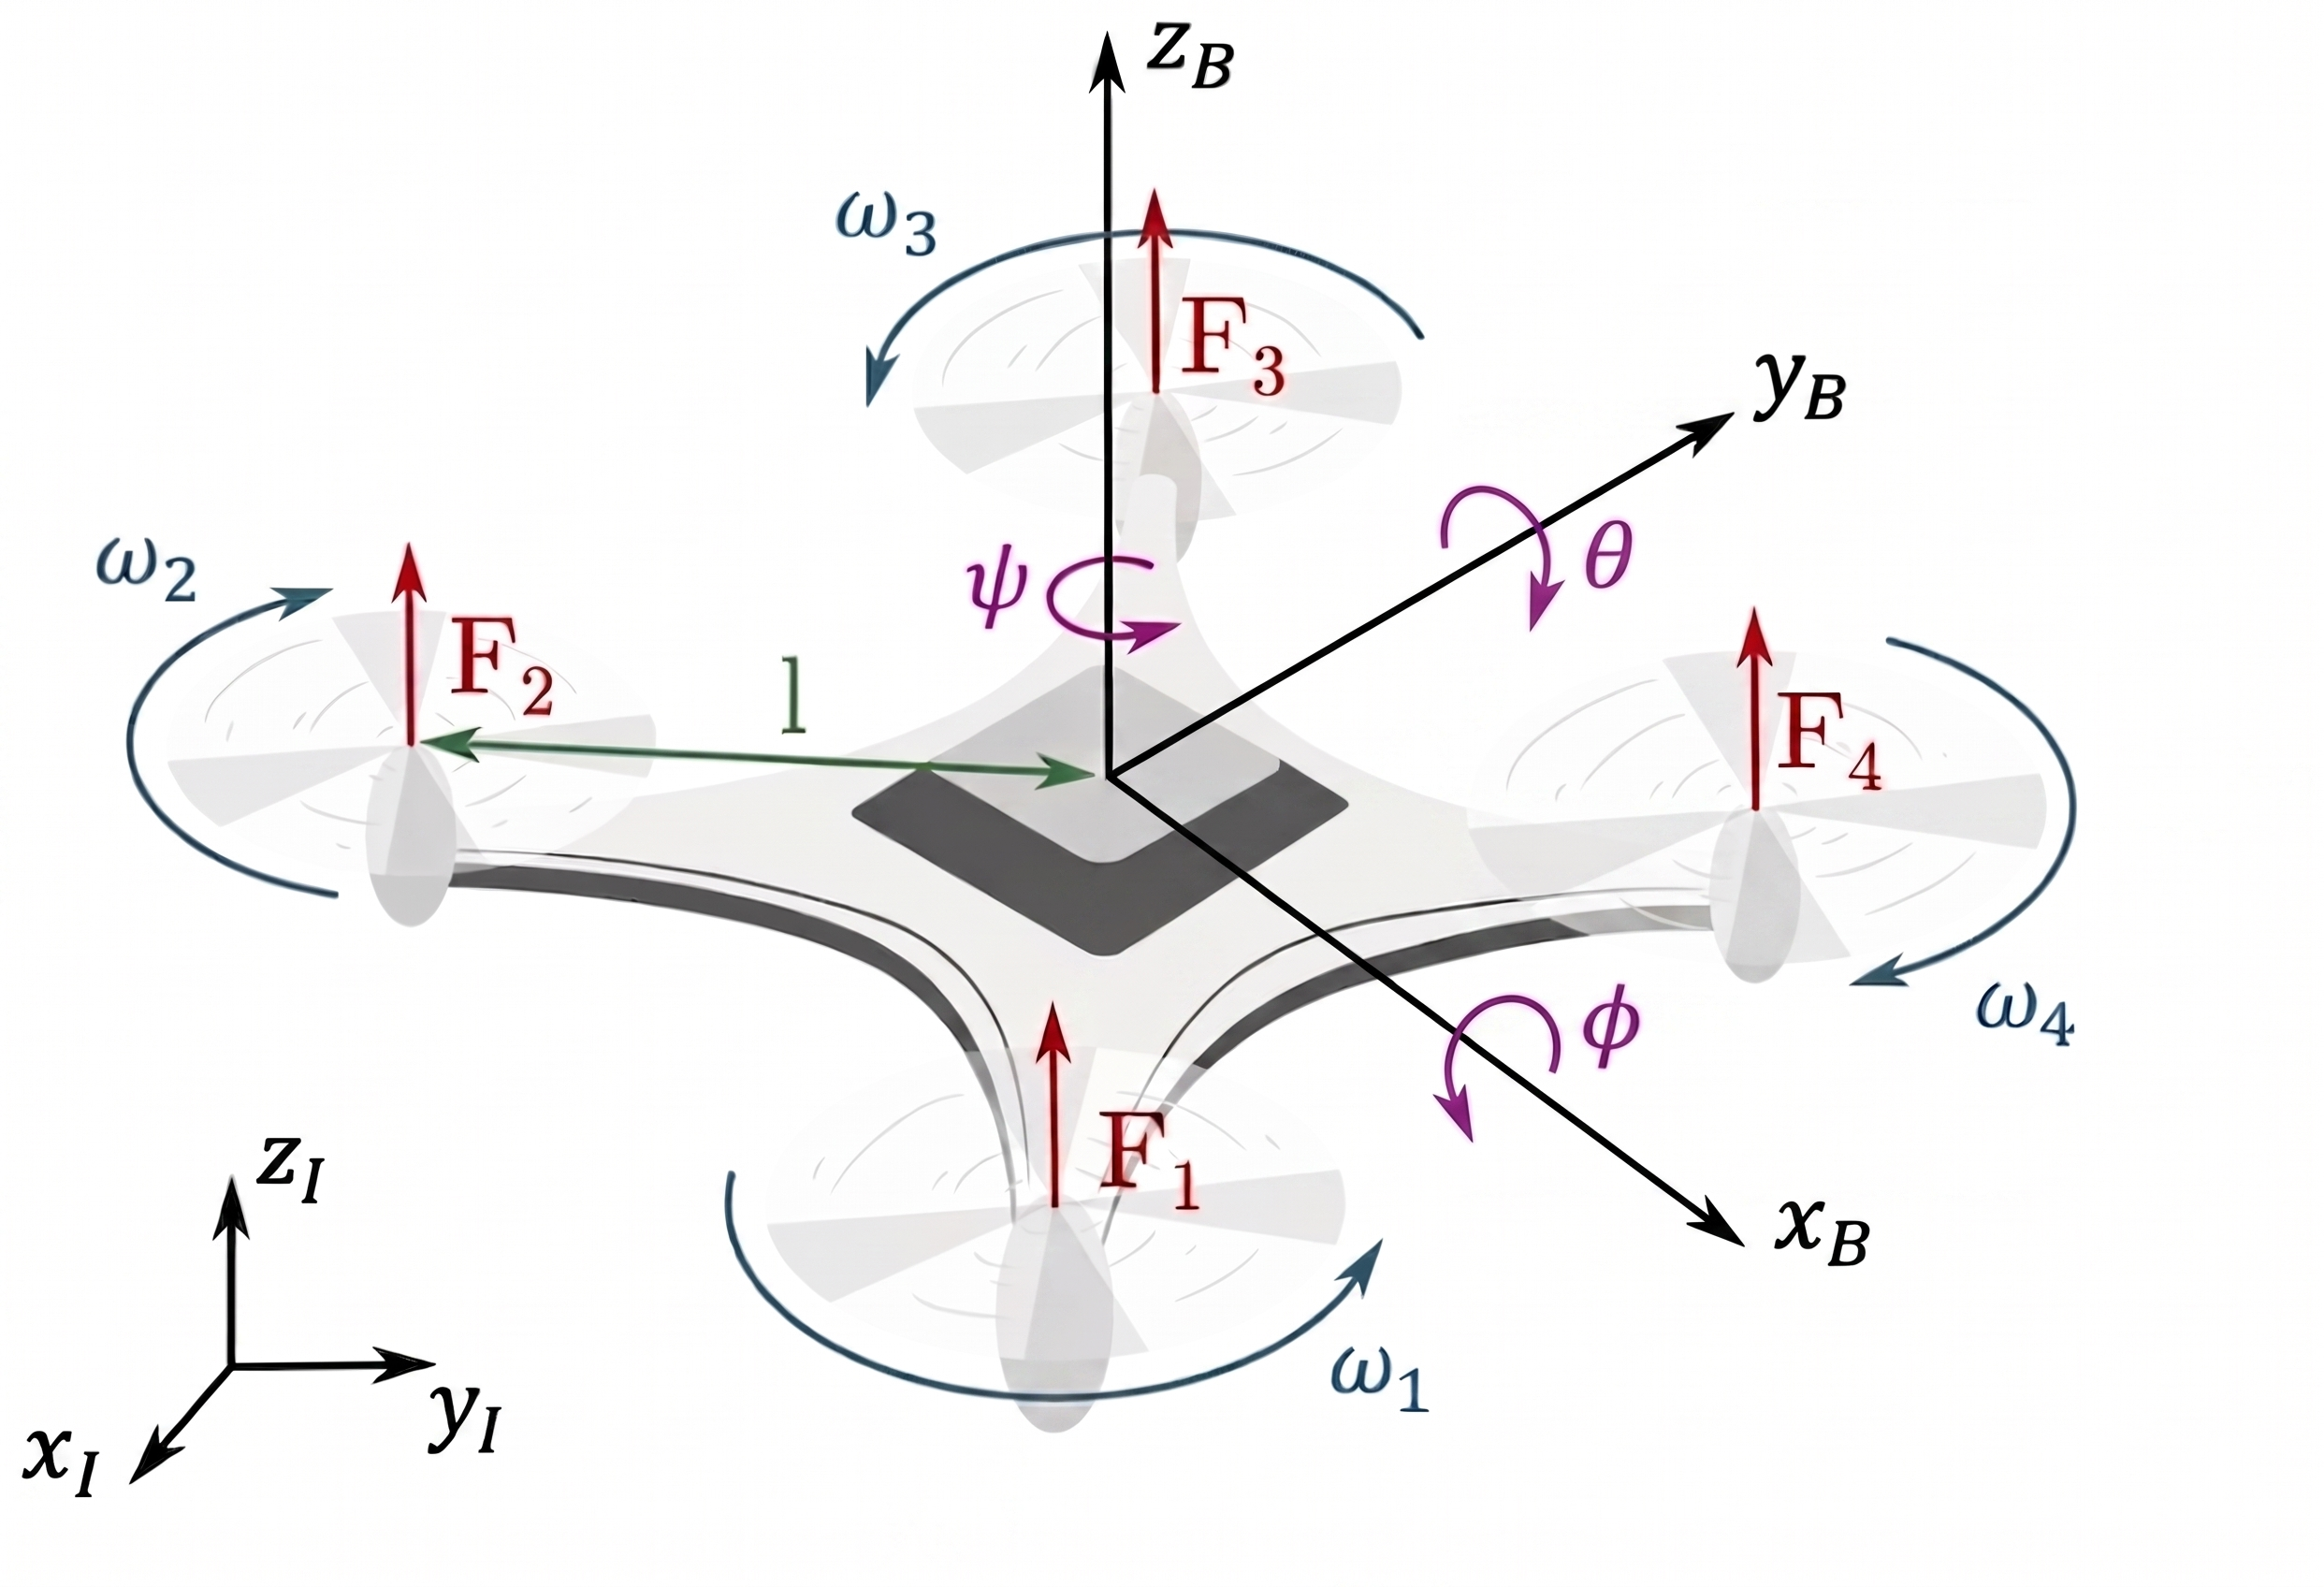
\includegraphics[width=\textwidth]{images/Quadcopter_Picture.png}
    \caption{Schematic representation of a quadcopter.}
    \label{fig:quadcopter}
\end{figure}

\subsection{Crazyflie Cascade PID Architecture}
\subsection{Neural Network Control Policy}
\subsection{Back-Propagation Through Time and Curriculum Reset}
\subsection{Model-Agnostic Meta-Learning (MAML)}

% =====================================================
\section{Simulation Environment}
\subsection{gym-pybullet-drones}
\subsection{Dynamics Model Comparison}
\subsection{Crazyflie Firmware Integration}

% =====================================================
\section{Sim-to-Real Validation}
\subsection{Experimental Setup}
\subsection{Flowdeck vs Lighthouse}
\subsection{Circle Trajectory: Simulation vs Reality}

% =====================================================
\section{Learning Classic Regulation}
\subsection{NN-PID Hybrid Architecture}
\subsection{Training}
\subsection{Simulation Results}
\subsection{Real-World Results}

% =====================================================
\section{MAML for Offset Mass Compensation}
\subsection{Task Definition}
\subsection{Training}
\subsection{Results}

% =====================================================
\section{Conclusion}

\newpage
% %%%%%%%%% REFERENCES SECTION %%%%%%%%%
\bibliographystyle{ieeetr}
% This is the link to the refereces file. 
\bibliography{main}

\end{document}

